\chapter{Banding instability of active hard needles}\label{ch06_active_matter}
In this chapter, I study how the interplay between activity, a local
nonconservative driving force, and interparticle interactions leads to
collective motion and self-assembly~\cite{marchetti_hydrodynamics_13}.  I will
present a general dynamical density functional theory for studying active
systems, and apply the theory to a model system of self-propelled needles. 

% From paper
Active matter refers to collections of interacting particles which can convert
an energy source into a propulsive force. These systems exhibit collective
motion, self-assembly, nonequilibrium dynamical phases, anomalous fluctuations,
and unusual mechanical responses on length scales ranging from microns to
meters~\cite{marchetti_hydrodynamics_13}. Some examples are cytoskeletal
filaments and motor proteins~\cite{nedelec_selforganization_97}, animal
flocks~\cite{cavagna_scalefree_10}, bacterial swarms~\cite{zhang_collective_10,
  cisneros_dynamics_11,thutupalli_directional_15}, crawling
cells~\cite{rappel_selforganized_99}, and vibrated granular
particles~\cite{kudrolli_swarming_08, narayan_longlived_07,
  deseigne_collective_10}.  Since the initial work by
Vicsek~\cite{vicsek_novel_95}, the study of active systems has illuminated
features not found in equilibrium fluids, such as collective
motion~\cite{toner_longrange_95, toner_flocks_98, peruani_kinetic_13,
  peruani_nonequilibrium_06, wensink_emergent_12, mccandlish_spontaneous_12,
  gregoire_onset_04, chate_collective_08, ginelli_largescale_10,
  deseigne_collective_10, kuan_hysteresis_15, gao_multiscale_15,
  mishra_fluctuations_10, gopinath_dynamical_12, peshkov_nonlinear_12} and giant
number fluctuations~\cite{simha_hydrodynamic_02, ramaswamy_active_03,
  chate_collective_08, chate_simple_06,
  mccandlish_spontaneous_12,menzel_unidirectional_13}.  Certain active
properties such as laning~\cite{sutterlin_dynamics_09, leunissen_ionic_05,
  vissers_lane_11}, phase separated clusters or flocks~\cite{palacci_living_13,
  theurkauff_dynamic_12,buttinoni_dynamical_13}, and large density
fluctuations~\cite{narayan_longlived_07, zhang_collective_10} have been
experimentally realized.

Anisotropic active particles fall into three main classes depending on the
polarity of their interactions and activity: polar active (polar activity and
interactions), apolar active or active nematic (apolar activity and
interactions), and self-propelled (polar activity and apolar
interactions)~\cite{baskaran_selfregulation_12,marchetti_hydrodynamics_13}. 

Self-propelled rods (SPRs) exhibit the hallmark active matter properties while
having minimal features: excluded volume interactions and driving.  This chapter
focuses on self-propelled hard needles (infinitesimally thin rods) in a 2D dry
system (a Brownian heat bath lacking hydrodynamic coupling between particles,
but providing random kicks and a drag force acting on the
particles)~\cite{marchetti_hydrodynamics_13}. 

Previous theoretical work has been of two flavors: phenomenological equations
based on symmetries~\cite{toner_longrange_95, toner_flocks_98} and
course-grained models of microscopic interactions~\cite{bertin_hydrodynamic_09,
  baskaran_hydrodynamics_08, baskaran_enhanced_08, liverpool_instabilities_03}.
Hydrodynamic theories of self-propelled rods have studied the effects of apolar
(nematic) interaction for steric~\cite{baskaran_hydrodynamics_08} and
Yukawa~\cite{wensink_aggregation_08} repulsion, activity-modified
interactions~\cite{baskaran_enhanced_08}, and a phenomenological polar
interaction~\cite{mishra_fluctuations_10}. These theories predicted instability
of the nematic state~\cite{baskaran_hydrodynamics_08}, enhanced diffusion and
modified interactions based on activity~\cite{baskaran_enhanced_08}, clustering
near confining walls~\cite{wensink_aggregation_08}, and a mapping of SPRs to
active nematics~\cite{baskaran_selfregulation_12}.  Furthermore,
infinitesimally thin SPRs display rich dynamical phases which include an
inhomogeneous band state predicted by theory~\cite{baskaran_hydrodynamics_08,
  baskaran_selfregulation_12} and demonstrated in
simulations~\cite{ginelli_largescale_10, kuan_hysteresis_15}.

In our work, we study self-propelled
hard needles in a 2D dry periodic system using dynamical density functional theory
(DDFT)~\cite{evans_nature_79, marconi_dynamic_99, marconi_dynamic_00,
  archer_dynamical_04}.  Our model begins with the same microscopic model and
approach as \cref{baskaran_hydrodynamics_08}.  However, unlike previous work, we
solve the full system of equations instead of 
approximate equations for 
concentration, polar order, and nematic order. We connect past work to DDFT to
clarify some confusion in the literature, describe how the DDFT framework
lends itself to studying other active systems, and suggest improvements
for the theory. We numerically solve the working equations to find a nematic band
at high driving stabilized by inhomogeneous polar order.  Our results
suggest that mapping SPRs to active
nematics~\cite{baskaran_selfregulation_12} is not completely valid, even
without a modified interaction from activity as in
\cref{baskaran_nonequilibrium_10,baskaran_enhanced_08}, because an active
nematic cannot possess polar order. Finally, by comparing to
simulations, we address the strengths and limitations of our theory.

%%%%%%%%%%%%%%%%%%%%%%%%%%%%%%%%%%%%%%%%%%%%%%%%%%%%%%%%%%%%%%%%%%%%%%%%
\section{Microscopic interactions}
%%%%%%%%%%%%%%%%%%%%%%%%%%%%%%%%%%%%%%%%%%%%%%%%%%%%%%%%%%%%%%%%%%%%%%%%
Our system contains $N$ infinitely-thin needle shaped particles of length $L$ in
a two-dimensional periodic Brownian heat bath of length $L_{\tx{box}}$. The
particles experience forces from steric interactions, driving along their
director $ \hat{\bm{u}} $, and random kicks and drag from the solution. Our
Brownian heat bath is `dry': there is no momentum conservation (\textit{i.e.},
no hydrodynamic interactions).

%%%%%%%%%%%%%%%%%%%%%%%%%%%%%%%%%%%%%%%%%%%%%%%%%%%%%%%%%%%%%%%%%%%%%%%
\subsection{Langevin equations of motion}

Our simulations directly integrate the microscopic equations of motion.  The
Brownian dynamics of the $i^{th}$ particle's position $\bm{r}_i$ and orientation
$ \hat{ \bm{u} }_i = [ \cos \theta_i, \sin \theta_i ] $ is described by the
overdamped Langevin equations
% Position
\begin{gather}
  \label{eqn:lang_pos}
  \frac{d \bm{r}_i}{dt} = \boldsymbol{\zeta}_{i}^{-1} 
  \left[ -\nabla_i V(\bm{r}^{N}, \hat{\bm{u}}^{N} ) 
  + F_D \hat{\bm{u}}_{i} + \bm{\xi}_i(t) \right],\\
  \label{eqn:lang_or}
  \frac{d \hat{\bm{u}}_i}{dt} = \frac{1}{\zeta_i^{R}} 
  \left[ -\frac{\partial}{\partial \theta_i}
  V(\bm{r}^{N}, \hat{\bm{u}}^{N} ) + \xi^R_i(t) \right],
\end{gather}
%
where $ \bm{r}^{N} = [\bm{r}_1, \bm{r}_2, \ldots, \bm{r}_N ] $ and $
\hat{\bm{u}}^{N} = [ \hat{\bm{u}}_1, \hat{\bm{u}}_2, \ldots,\hat{\bm{u}}_N] $
are the $2N$ dimensional position and orientation vectors, $\bm{\zeta}$ the
spatial friction tensor, $\zeta^{R}$ the rotational drag, $V$ the potential
energy, $F_D$ the driving force, and $\bm{\xi}$ and $\xi^R$ the spatial and
rotational noise terms. We have ignored hydrodynamic interactions but have
included anisotropy due to the particle geometry in the mobility $
\zeta^{-1}_{\alpha,\beta} = \zeta^{-1}_{\parallel} \hat{u}_{\alpha}
\hat{u}_{\beta} + \zeta^{-1}_{\perp} (\delta_{\alpha,\beta} - \hat{u}_{\alpha}
\hat{u}_{\beta} ) $ where $\alpha$, $\beta$ label Cartesian coordinates. The
noise terms are Gaussian-distributed and uncorrelated in time, spatial
coordinates, and between particles
% Noise
\begin{gather}
  \langle \xi_{i,\alpha}( t ) \xi_{j,\beta} ( t') \rangle = 
  2 \zeta_{\alpha \beta}  k_B T \delta_{i j} 
  \delta_{\alpha \beta} \delta(t-t'), \\
  \langle \xi_{i}^{R}(t) \xi_{j}^{R} ( t') \rangle = 2 \zeta_{R} 
  k_B T \delta_{i j} \delta(t-t').
\end{gather}
%
The potential energy depends solely on excluded volume
interactions between particles
%
\begin{equation}
  V(\bm{r}^{N}, \hat{\bm{u}}^{N} ) = 
  \sum_{i \neq j } 
  V(\bm{r}_i - \bm{r}_j,\hat{\bm{u}}_{i}, \hat{\bm{u}}_{j} ) = 
  \begin{cases}
    \infty , & \text{if particles $i,j$ overlap} \\
    0 , & \text{no overlap} 
  \end{cases}.
\end{equation}
%
Unlike some previous work~\cite{baskaran_enhanced_08,
  baskaran_nonequilibrium_10, baskaran_selfregulation_12}, we did not include a
modified potential due to momentum transfer in collisions in our model; all
particle-particle effects are included in the interaction potential.  The
simulation methods we implemented to solve the equations are described in
\cref{frenkel_evidence_85, tao_brownian_05, tao_isotropicnematic_06,
  mccandlish_spontaneous_12, lowen_brownian_94, weeks_role_71,
  hansen_theory_06}.  All simulations in this project were done by Hui-Shun Kuan
and are included in this thesis for completeness.

%%%%%%%%%%%%%%%%%%%%%%%%%%%%%%%%%%%%%%%%%%%%%%%%%%%%%%%%%%%%%%%%%%%%%%%
\section{Continuum equations}
%%%%%%%%%%%%%%%%%%%%%%%%%%%%%%%%%%%%%%%%%%%%%%%%%%%%%%%%%%%%%%%%%%%%%%%
Starting from the microscopic equations of motion (\eqnref{eqn:lang_pos},
and~\ref{eqn:lang_or}), we are interested in arriving at a continuum continuity
equation for the one-particle density $ \rho(\bm{r}, \hat{ \bm{u} },t) $,
%
\begin{equation}
  \label{eqn:continuity}
  \frac{\partial \rho( \bm{r}, \hat{\bm{u}}, t )}{\partial t} 
  = -\bm{\nabla} \cdot \bm{j} ( \bm{r}, \hat{\bm{u}}, t ),
\end{equation}
%
where $\bm{j}$ is the flux.  The one-body density, or density profile, is the
noise ensemble average of the instantaneous microscopic density operator
$\rho(\bm{r}) = \ev{\sum_i \delta( \bm{r} - \bm{r}_i )}$. The density operator
depends on the instantaneous positions of every particle for a given experiment
or simulation while the density profile is an average of $\hat{\rho}$ over
identical initial conditions but with different realizations of the noise
$\xi$, \textit{i.e.}, one experiment tells you the behavior of $\hat{\rho}$,
and averaging over many experiments describes $\rho$.  The density profile is
the probability density of finding a particle at location $\bm{r}$ pointing in
direction $ \hat{ \bm{u} } $ irrespective of the locations of other particles.
Unlike solving for the dynamics of the density propagator or a course-grained
density, the temporal evolution is deterministic~\cite{archer_dynamical_04a}. 

In our system, there can be fluxes from diffusion, interactions, and driving. We
can separate the local driving flux $\bm{j}^{D}$ from the diffusive and
interaction flux $\bm{j}^{\mathcal{F}}$.  The driving term is given by
%
\begin{equation}
  \bm{j} ^ {D}  = \zeta^{-1} F_D \hat{\bm{u}} 
  \rho( \bm{r}, \hat{\bm{u}}, t).
\end{equation}
%
To find $\bm{j}^{\mathcal{F}}$ in terms of microscopic interactions, we
implemented DDFT\@.

% Additional paragraph not in paper connect DDFT to microscopic models
In the introduction of this thesis, we discussed a continuity equation for
noninteracting particles, \textit{i.e.}, the diffusion equation. Our goal here
is to present a continuity equation for the density of interacting particles
starting from microscopic interactions. Arriving at a continuity equation for
the $N$ particle phase space density starting from the Langevin
equation (\textit{i.e.}, the Smoluchowski equation) is straightforward (see
\appxref{appx:smoluchowski}).  However, this $2N$ dimensional (for 2D) phase
space density is not only numerically intractable for large systems, it does not
correspond to an experimentally measurable quantity. Dynamical density
functional theory allows us to go from the Smoluchowski equation to a closed
equation for the one-body density.  We will avoid these details here, but the
steps are laid out in \appxref{appx:ddft}.  In the following section, we will
present the DDFT equation and discuss the implementation for our active needle
system.

\subsection{Dynamical density functional theory}

Dynamical density functional theory (DDFT) is a technique to obtain the temporal
evolution of the one-body density~\cite{marconi_dynamic_99, marconi_dynamic_00,
  archer_dynamical_04}.  By assuming that correlations out of equilibrium are of
the same form as equilibrium correlations but at the nonequilibrium density
$\rho(\bm{r},t)$~\cite{archer_dynamical_04}, DDFT casts the temporal evolution
of density in terms of functional derivatives of the free energy
%
\begin{equation}
  \bm{j} ^ {\mathcal{F}} = 
  -\bm{\zeta}^{-1} \left(\rho( \bm{r}, \hat{\bm{u}}, t )
  \bm{\nabla} \frac{\delta \mathcal{F}[ \rho ]}
  {\delta \rho( \bm{r}, \hat{\bm{u}}, t ) } \right).
\end{equation}
%
The free energy can be separated into an ideal gas term and an
excess term from interactions, $\mathcal{F} = \mathcal{F}^{\tx{id}} +
\mathcal{F}^{\tx{ex}}$. The ideal gas term which leads to diffusion is
exact~\cite{hansen_theory_06}.  To approximate the excess free energy, we used
the second virial approximation, which Onsager originally used to 
predict the isotropic-nematic (IN) transition in three
dimensions~\cite{onsager_effects_49}.  This functional 
describes the equilibrium phase behavior, can be connected directly to
microscopic interactions, and is numerically tractable.  By truncating the
virial expansion at the second term, the approximate excess free energy is
%
\begin{equation}
  \label{eqn:mayer}
  \mathcal{F}^{\tx{ex}} = - \frac{k_B T}{2} \int 
  \dif \bm{r} \dif \hat{\bm{u}} \dif \bm{r}' \dif \hat{\bm{u}}'
  F_{M}(\bm{r}-\bm{r}',\bm{u},\bm{u}') 
  \rho(\bm{r},\bm{u},t) \rho(\bm{r}',\bm{u}',t) ,
\end{equation}
%
where $ F_{M}(\bm{r}-\bm{r}',\bm{u},\bm{u}') =  \exp(-\beta V(\bm{r} -
\bm{r}',\hat{ \bm{u} }, \hat{ \bm{u} }') )- 1 $ is the Mayer
function~\cite{hansen_theory_06}.  The second-virial approximation amounts to
approximating the direct pair correlation with the Mayer
function~\cite{hansen_theory_06}.  For more information on the second virial
approximation, see~\appxref{appx:2nd_virial}.

While ignoring higher order terms works well in 3D, this approximation can lead
to dubious quantitative results in 2D~\cite{kayser_bifurcation_78,
  frenkel_evidence_85}.  In the absence of driving, the second virial
approximation predicts the isotropic-nematic transition at concentration
$c=N/L_{\tx{box}}^2 =\frac{3 \pi}{2} \sim 4.71$~\cite{kayser_bifurcation_78}
while simulation finds a value of $c \sim 7.25 $~\cite{frenkel_evidence_85,
  bates_phase_00}.   Qualitatively, the second virial only
accounts for two-particle interactions.  Higher order virial coefficients are
more important in two than three dimensions~\cite{frenkel_evidence_85} because
multiple particle overlaps are more likely at a fixed concentration in two
dimensions.  
However, we believe that this approximation can qualitatively
represent the nonequilibrium phase behavior of hard needles because it correctly
accounts for the phases in the equilibrium system.  Note, \eqnref{eqn:mayer}
cannot account for finite width effects in 2D, and therefore only describes needles
\appxrefp{appx:2nd_virial}.

By plugging in the flux and taking the functional derivatives,  we obtain our
working equation of motion
%
\begin{equation} 
  \label{eqn:working}
  \begin{aligned}
    \partial_t \rho(\bm{r}, \hat{\bm{u}}, t) &= 
    \bm{\nabla} \cdot  \bm{D} \bm{\nabla} \rho (\bm{r}, \hat{\bm{u}}, t) 
    - \bm{\nabla}  \cdot \bm{\zeta}^{-1} F_D 
    \hat{\bm{u}} \rho( \bm{r}, \hat{\bm{u}}, t ) \\
    &-\bm{\nabla} \cdot  \bm{D}  \rho (\bm{r}, \hat{\bm{u}}, t)
    \bm{\nabla}
    \int  F_{M}(\bm{r} - \bm{r}',\hat{\bm{u}}, \hat{\bm{u}}') 
    \rho(\bm{r}',\hat{\bm{u}}',t)  \dif \bm{r}' \dif \hat{\bm{u}}',
  \end{aligned} 
\end{equation}
%
where
\begin{equation}
  \bm{D} =
\left[
\begin{array}{c c c}
  \bm{D}_T & \rvline & 0\\
\midrule
 0  & \rvline & D_R
 \end{array}
\right].
\end{equation}
%
is a block diagonal matrix separated into its translational component $
D_T^{\alpha \beta} = D_{\parallel} \hat{u}_{\alpha} \hat{u}_{\beta} + D_{\perp}
(\delta_{\alpha \beta} - \hat{u}_{\alpha} \hat{u}_{\beta} ) $ and rotational
component $D_R$. In principle, activity can influence
$D_{\parallel}$~\cite{baskaran_enhanced_08} and interactions can introduce a
density dependent effect on diffusion~\cite{doi_theory_88}. We neglect these
effects.  For passive infinitely thin rods in the low density limit, $
D_{\parallel} = 2 D_{\perp} =  \frac{2  k_B T}{\zeta} = 2 D_0$ and  $D_R =
\frac{6 k_B T}{ \zeta l^2} $ where $\zeta$ is the drag coefficient between the
particle and solution~\cite{doi_theory_88}. Note that in \eqnref{eqn:working},
there are no phenomenological parameters. Our tunable parameters here are the
same as the microscopic model: the driving force and the concentration. 

%%%%%%%%%%%%%%%%%%%%%%%%%%%%%%%%%%%%%%%%%%%%%%%%%%%%%%%%%%%%%%%%%%%%%%%
\subsection{Pseudospectral numerical scheme} 
To numerically solve
\eqnref{eqn:working}, we implemented a pseudospectral
method~\cite{fornberg_practical_98}.  Complex exponentials form a complete basis
for the density profile due to the periodicity of the system. The implemented
spectral method involves Fourier transforming the spatial coordinates to
momentum space, $ \rho(\bm{X},t) \rightarrow  \tilde{ \rho } (\bm{k},t ) $
where $\bm{X} = [x,y,\phi]$ and $\bm{k} = [k_x, k_y, k_m]$, and integrating in
time.  All diffusive terms linear in $\tilde{\rho}$ are included in
a linear propagator $M$ while the interaction and driving terms are included
in a non-linear term $\psi$.  In momentum space, our equation is
%
\begin{equation}
  \label{eqn:k2solve}
  \frac{\partial \tilde{\rho} ( \bm{k}, t )} {\partial t} = 
  M  \tilde{\rho} ( \bm{k}, t ) + 
  \tilde{\psi} ( \bm{k}, t ).
\end{equation}
%
We calculate derivatives and convolutions in momentum space and
products in real space.  We calculate the terms in \eqnref{eqn:working} at a
given time step using the transforms until we get the 1st order ODE in
\eqnref{eqn:k2solve}. The numerical integration of \eqnref{eqn:k2solve} gives
%
\begin{equation}
  \tilde{\rho} ( \bm{k}, t + \delta t )
  \approx e^{M \delta t}  \tilde{\rho}( \bm{k}, t ) +   
  \delta t \phi( M \delta t ) \tilde{\psi}( \bm{k}, t ),
\end{equation}
%
where $\phi(x) = (\exp(x) - 1)/x $. If the propagator is diagonal, we can easily
calculate the exponential.  In the case where the operator is not diagonal, we
used expokit~\cite{sidje_expokit_98} to handle the exponential of the sparse
matrix $M$. In principle, the driving force terms should be put in the linear
propagator $M$. However, it is more computationally efficient to put it in the
nonlinear term to make $M$ diagonal. We set
$D_{\parallel} = D_{\perp}$ to make $M$ diagonal to further simplify the
numerics and increase computational performance for the results in this chapter.
We verified that the dynamics are not significantly altered by keeping
anisotropies in the equations (results not shown), and this assumption has been
used previously~\cite{mishra_fluctuations_10}.

We scale length by rod length $L$, energy by $k_B T$, and time by the
diffusion time $\tau = L^2 / D_0$. The box size was fixed at $L_{\tx{box}}
= 10$, and we use $N_x = N_y = N_{\phi} = 160$ gridpoints. We
scale concentration by the average excluded area per particle $c^* = bc =
\frac{ N L^2 }{ \pi L_{\tx{box}}^2 } $. In our scaling scheme, the driving force
is equivalent to the \peclet~number $\pe = \frac{ L \zeta^{-1} F_D }{ D } \equiv
F_D$ and the names are used interchangeably.  The initial condition was varied,
but typically an isotropic or nematic with random plane wave perturbations was
used.

%%%%%%%%%%%%%%%%%%%%%%%%%%%%%%%%%%%%%%%%%%%%%%%%%%%%%%%%%%%%%%%%%%%%%%%
\section{Results}
%%%%%%%%%%%%%%%%%%%%%%%%%%%%%%%%%%%%%%%%%%%%%%%%%%%%%%%%%%%%%%%%%%%%%%%
The dynamical density functional equation \eqnrefp{eqn:working} was numerically
integrated for varying initial condition, concentration, and driving
force. For concentration below the equilibrium IN transition $c^*<c_{IN}$,
the system decays to a homogeneous isotropic regardless of driving
and initial condition.  For $c^* > c_{IN}$, a homogeneous nematic is
stable at low activity and high concentration. These match the linear
instability predictions due to splay deformations for this specific
system~\cite{baskaran_hydrodynamics_08} as well as a similar behavior in active
nematic systems~\cite{baskaran_selfregulation_12, putzig_phase_14}. 

From $\rho(\bm{r}, \hat{ \bm{u} }, t)$, we compute the local concentration and
polar and nematic order parameters 
%
\begin{align}
C(\bm{r},t) &= \int \dif  \hat{\bm{u}} \,
  \rho( \bm{r}, \hat{\bm{u}}, t ) \\
P_i (\bm{r},t) &= \frac{\int \dif  \hat{\bm{u}} \,
  \hat{u}_i \rho( \bm{r}, \hat{\bm{u}},t )}{C( \bm{r}, t )} \\
N_{i j} (\bm{r},t) &= \frac{2 \int \dif  \hat{\bm{u}} \,
  \left( \hat{u}_i \hat{u}_j - \frac{1}{2} \delta_{ij} \right)
  \rho( \bm{r}, \hat{\bm{u}},t )}{C( \bm{r}, t )}.
\end{align}
%
The degree of alignment at a given location is given by the magnitude of the
polar order $ P(\bm{r},t) =  \|{ \bm{P}(\bm{r},t) } \|$, and the largest
eigenvalue value of the nematic tensor $ N(\bm{r},t) =
\max{E_{\lambda}(\bm{N})}$. We also scaled the local concentration by the
average excluded area.

%%%%%%%%%%%%%%%%%%%%%%%%%%%%%%%%%%%%%%%%%%%%%%%%%%%%%%%%%%%%%%%%%%%%%%%
\subsection{Banding instability}
% figure 1
\begin{figure}[!b]
	\centering
  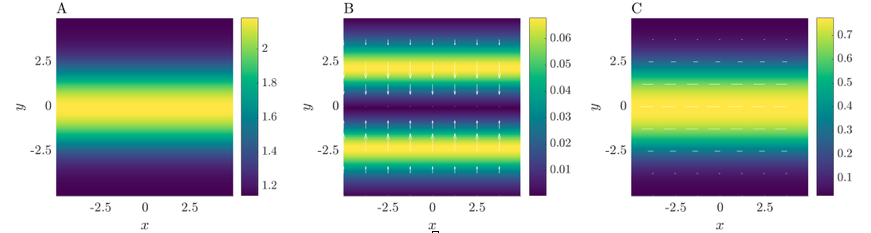
\includegraphics[width=1.00\textwidth]{figs/ch04_active/band_example_paper.png}
  \caption[Banding instability]
  {(A) Concentration, (B) polar order, and (C) nematic order 
    as a function of position for the steady band
    state with concentration $c^* = 1.55$ and \peclet~number $\pe = 10$.
    Magnitude is indicated by color and order parameter director arrows are 
    shown in white. The dense inhomogeneous nematic band is orientated parallel 
    to the local nematic director and is stabilized by inwardly pointing polar
    edges.}\label{fig:band}
\end{figure}
% end figure
% figure 2
\begin{figure}[!t]
	\centering
  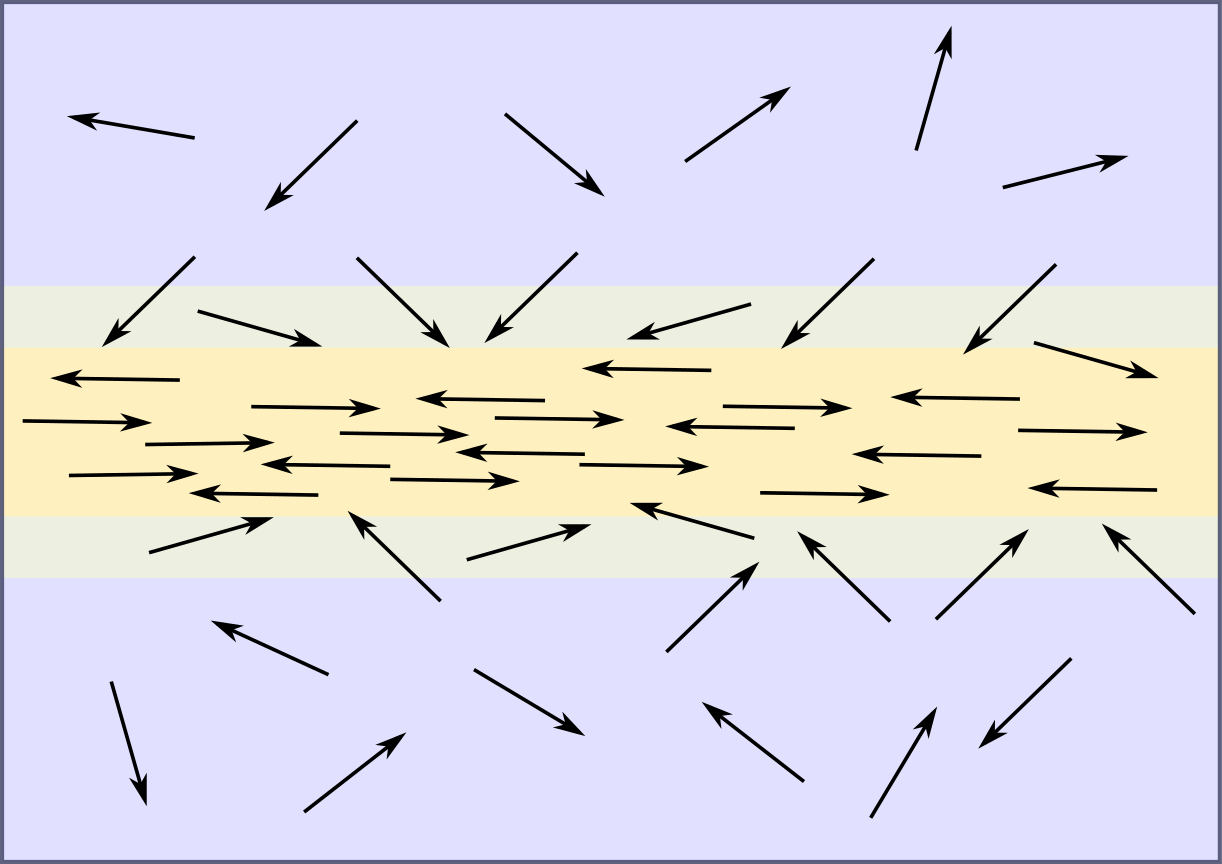
\includegraphics[width=0.50\textwidth]{figs/ch04_active/band_cartoon_paper.png}
  \caption[Band stability schematic]
  {Band stability schematic. The dense nematic band corresponds to
    perfectly mixed counterpropagating needles. The band is supported by a polar
    edge. The polar order is pointing in toward the band because it is equally
    likely for a particle to be pointing along either direction of the band.
    Outside the
    polar region, there is a sparse isotropic gas.}\label{fig:band_cartoon}
\end{figure}
% end figure


The SPR system has a banding instability for concentration above the IN
transition at sufficient driving \figrefp{fig:band}. The band of high concentration
and nematic order is surrounded by a low density isotropic gas
\figrefp{fig:band_cartoon}.  The band is oriented parallel to the nematic
director, and, unlike active nematics which cannot possess a polar
state~\cite{putzig_phase_14}, the stability in this system is due to a polar
band. The dense
nematic band can be understood as a perfectly mixed collection of
counterpropagating particles.

Diffusion and interactions generate fluxes that dissolve the band while  an
inward flux towards the band's center from  activity stabilizes the band.
Qualitatively, the inward active flux arises because the activity drives rods in
the nematic band along the band while it propels rods in the gas in all
directions. Thus, it is more likely for a particle to join the band from the gas
than to leave.  This creates a polar strip outside the band that supports the
structure.  Another interpretation of this instability is a competition between
splay and bend deformation at the boundaries of the
band~\cite{baskaran_hydrodynamics_08}.  In our description, this can interpreted
as an active flow of particles into a band with equal probability of pointing in
either direction along the band.

% figure 3
\begin{figure}[!b]
	\centering
  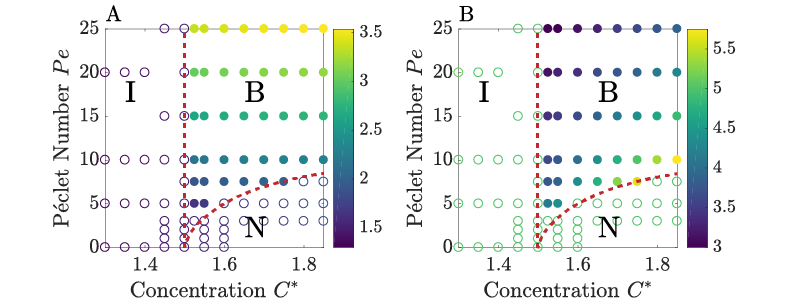
\includegraphics[width=1.0\textwidth]{figs/ch04_active/phase_diagram_paper.png}
  \caption[Dynamical phase diagram]
  {Dynamical phase diagram for (A) max band concentration and (B) peak
    concentration full width half max as a function of \peclet~number and
    concentration. There are three distinct phases: homogeneous isotropic (I),
    homogeneous nematic (N), and inhomogeneous band (B). The dashed red lines
    separate the homogeneous and inhomogeneous regions.}\label{fig:phase_diagram}
\end{figure}
% end figure

Above a critical driving and density, shown in dashed red lines in
\figref{fig:phase_diagram}, the system has a banding instability.  At fixed
\peclet~number, the band peak and width increase as density increases until the
band state is no longer stable. For increasing \peclet~number, the band peak
increase and width decreases. There is
no hysteresis or coexistence, suggesting that the band instability is second
order.

The homogeneous state is reentrant \figrefp{fig:phase_diagram}.  At low concentration a homogeneous isotropic is
stable. When the concentration exceeds the equilibrium IN value, a band state or
homogeneous nematic forms depending on the driving amplitude.  A band is formed
when fluctuations in the nematic order and driving cause an active flow
perpendicular to the global nematic order.  If this flow is large enough, it can
overcome diffusive fluxes to form a band state.  For higher nematic order and
low driving, the band is no longer stable because the active flux perpendicular
to the director is too small to support a band.

% figure 4
\begin{figure}[!t]
	\centering
  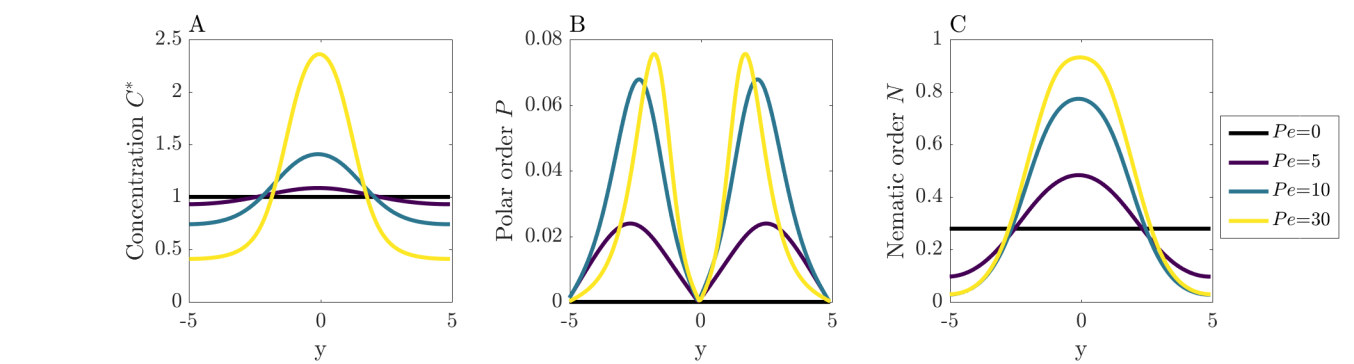
\includegraphics[width=1.00\textwidth]{figs/ch04_active/band_analysis_paper.png}
  \caption[Band structure]
  {A slice along the inhomogeneous direction for (A) concentration, (B) polar
    order, and (C) nematic order as a function of position for $c^* = 1.55$ and
    increasing \peclet~number.  For increasing \peclet~number, the band becomes
    more sharply peaked. The nematic order magnitude is tied to the
    concentration value while the polar order peak increases with \peclet~number
    to stabilize the band's structure.}\label{fig:band_analysis}
\end{figure}
% end figure

A slice along the inhomogeneous direction shows the band's structure
\figrefp{fig:band_analysis}. As driving increases, the band becomes more sharply
peaked in concentration and order parameter magnitude, and the inward flux
towards the band increases. We would expect a higher concentration gradient to
balance this effect, so the band gets thinner and more peaked. Since
the band thins with increasing driving, one may wonder if there is a
critical driving that destroys the band. We found that the numerics became
unstable (requiring more gridpoints to prevent a diverging solution) at high
driving, so this question remains a topic for further study.

%%%%%%%%%%%%%%%%%%%%%%%%%%%%%%%%%%%%%%%%%%%%%%%%%%%%%%%%%%%%%%%%%%%%%
\subsection{Connection to previous work}

In ref.~\cite{baskaran_selfregulation_12}, the authors demonstrated that a SPR
system an be mapped onto an active nematic.  A banding instability was predicted
through linear stability analysis and then demonstrated by solving the full
hydrodynamic equations of motion~\cite{putzig_phase_14}. Our results show that
this mapping is not exact because an active nematic system cannot possess the
observed polar band. Therefore, the argument that a band in this system is
stabilized by gradients in the nematic order~\cite{putzig_phase_14} is
incomplete.  While these systems demonstrate the same qualitative behavior,
different mechanisms stabilize the band.

It has been argued that banding is the result of dynamic self-regulation: the
density which controls the degree of order is convected by that order
parameter~\cite{baskaran_selfregulation_12, gopinath_dynamical_12}. While this
is true, it does not provide a microscopic description of stability. By starting
with a microscopic model, we can interpret bulk properties in terms of
microscopic behavior. In this case, a bulk band is stabilized because activity
creates a polar band of particles that produces an inward flux.

%%%%%%%%%%%%%%%%%%%%%%%%%%%%%%%%%%%%%%%%%%%%%%%%%%%%%%%%%%%%%%%%%%%%%%%
\subsection{Connection to simulations}
% figure 2
\begin{figure}[!b]
	\centering
  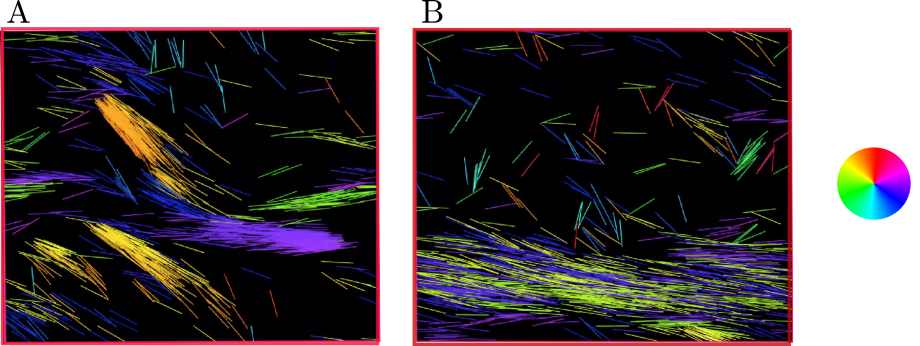
\includegraphics[width=0.75\textwidth]{figs/ch04_active/sim_flock_band_paper.png}
  \caption[Simulation snapshots]
  {Simulation results show two dynamical phases (A) flocking and (B)
    banding.  The flocking state is characterized by dynamic collective clusters
    that are long lived. The band state is a dense nematic composed of a 
    mixture of counterpropagating particles surrounded by a
    sparse isotropic gas. Unlike the DDFT results, the simulation band
    state is highly dynamic. Its center of mass fluctuates and can exhibit
    fluctuations in local polar along the band, \textit{i.e.}, the two
    groups of counterpropagating particles are not perfectly mixed.
    Simulation work done by Hui-Shun Kuan and used with
    permission.}\label{fig:sim_flock_band}
\end{figure}
% end figure 
Simulations of hard self-propelled rods with finite thickness have
showed flocking, turbulent-like states, and laning~\cite{wensink_emergent_12,
  kuan_hysteresis_15}. Our simulations, done by Hui-Shun Kuan, of
the infinitely thin rods show flocking \figrefp[A]{fig:sim_flock_band} and an
apparent band state \figrefp[B]{fig:sim_flock_band}.

Both the flocking and banding state are highly dynamic. With flocking, several
particles form a long-lived collective structure. Flocks are constantly forming
and disintegrating; they can collide with other flocks, break up, and form
again.  The band observed in simulation is also in constant motion.  It appears
to be two counterpropagating lanes passing through each other. The center of
mass fluctuates; the band will appear, break up, and form again. Unlike the
flocking state, there appears to be two definite, although shifting, regions
of high and low density in the band state.

The banding state has different behavior than previous laning
states~\cite{wensink_emergent_12, kuan_hysteresis_15, mccandlish_spontaneous_12,
  chakrabarti_dynamical_03}. A separation of counterpropagating lanes with 
finite width occurs from perpendicular flux due to collisions; particles
separate into lanes to minimize their collisions~\cite{chakrabarti_dynamical_03,
  kuan_hysteresis_15, mccandlish_spontaneous_12}. In our system, the rods are
infinitesimally thin. Thus, counterpropagating lanes can more easily pass
through each and mix without this perpendicular flux. Without this orthogonal
motion, a more mixed state of oppositely moving particles should be expected.

We can draw a few distinctions between simulation and DDFT\@. First, no flocking
state is evident in DDFT\@. One may expect to find a turbulent-like state
(fluctuations grow and decay in a seemingly chaotic fashion) in the DDFT
solutions, but none exists. The banding state also has differences: it is static
in DDFT but highly dynamic in simulation. The nematic order is the consequence
of two counterpropagating polar lanes happening to intersect than a stationary
(and evenly mixed) nematic.

What mechanisms produce these differences? First, 
DDFT solves for the ensemble average behavior of a
simulation.  If we were to consider all possible kicks a flock could receive, we
would need to average over all possible paths the flock could take, effectively
smearing the flock's density out. However, this doesn't seem to explain
everything: there is physics in these flocking states that our functional does
not describe.  For instance, particles inside a flock get jammed into a 
glass-like~\cite{kuan_hysteresis_15} polar state at high density. In DDFT, high
density fluctuations quickly decay, \textit{i.e.}, the functional can not
accurately describe jamming. Also, DDFT is notorious for not handling
fluctuations correctly~\cite{evans_nature_79, archer_interplay_11,
  malijevsky_sedimentation_13}.  For example, DDFT incorrectly characterizes the
center of mass fluctuations of a droplet~\cite{reguera_role_04}.

%%%%%%%%%%%%%%%%%%%%%%%%%%%%%%%%%%%%%%%%%%%%%%%%%%%%%%%%%%%%%%%%%%%%%%%
\section{Conclusions}
%%%%%%%%%%%%%%%%%%%%%%%%%%%%%%%%%%%%%%%%%%%%%%%%%%%%%%%%%%%%%%%%%%%%%%%
We have presented a dynamic density functional theory which demonstrates a
banding instability of active hard needles. We presented the framework as a
guide to apply this methodology to other active systems where DDFT has been
successful in describing the phase behavior of passive systems, \textit{e.g.},
a Gaussian core model~\cite{lang_fluid_00, dzubiella_meanfield_03} or soft
shoulder system~\cite{archer_quasicrystalline_13}.  Taking the
DDFT perspective, rather than considering a theory based on symmetry
arguments, can illuminate the strengths and weaknesses of the
approximations, and it can be directly compared to a microscopic model.

Using the second virial approximation, we have confirmed the banding instability
predicted in previous
work~\cite{baskaran_hydrodynamics_08,baskaran_selfregulation_12} by numerically
solving the full system of equations. We have laid out a dynamical phase diagram
in terms of microscopic parameters, the \peclet~number and concentration. Our
results are qualitatively similar to active nematics.  However, an inhomogeneous
band of polar order supports the structure. We have shown how the band peak
increases and becomes more compact as driving increases.   

We compared the DDFT results to simulations of the microscopic model. The
simulation shows rich dynamical phases including flocking and what appears to be
an analogous band structure. While we wouldn't expect the same long live
flocking states in an ensemble averaged density, \textit{i.e.}, in a theory for
the one body density, one may expect to more evidence of larger density
fluctuations. In DDFT at concentrations below $c_{IN}$, a homogeneous isotropic
is the stable state. While a flocking state could be argued to be isotropic and
homogeneous when averaging over many simulations, the flocking state has
different physical properties like pressure~\cite{kuan_hysteresis_15} than an
isotropic gas.  We believe that a functional that can incorporate the physics
seen in simulations (like jamming) is the key to a theory that more closely
matches simulation results.  One such example would be fundamental measure
theory~\cite{rosenfeld_freeenergy_90} although numerically this may be a
challenge.
